%   Filename    : chapter_4.tex 
\section*{Chapter 4}
\section{Preliminary Results/System Prototype}
\subsection{Original Ontology}
\begin{figure}
    \centering
    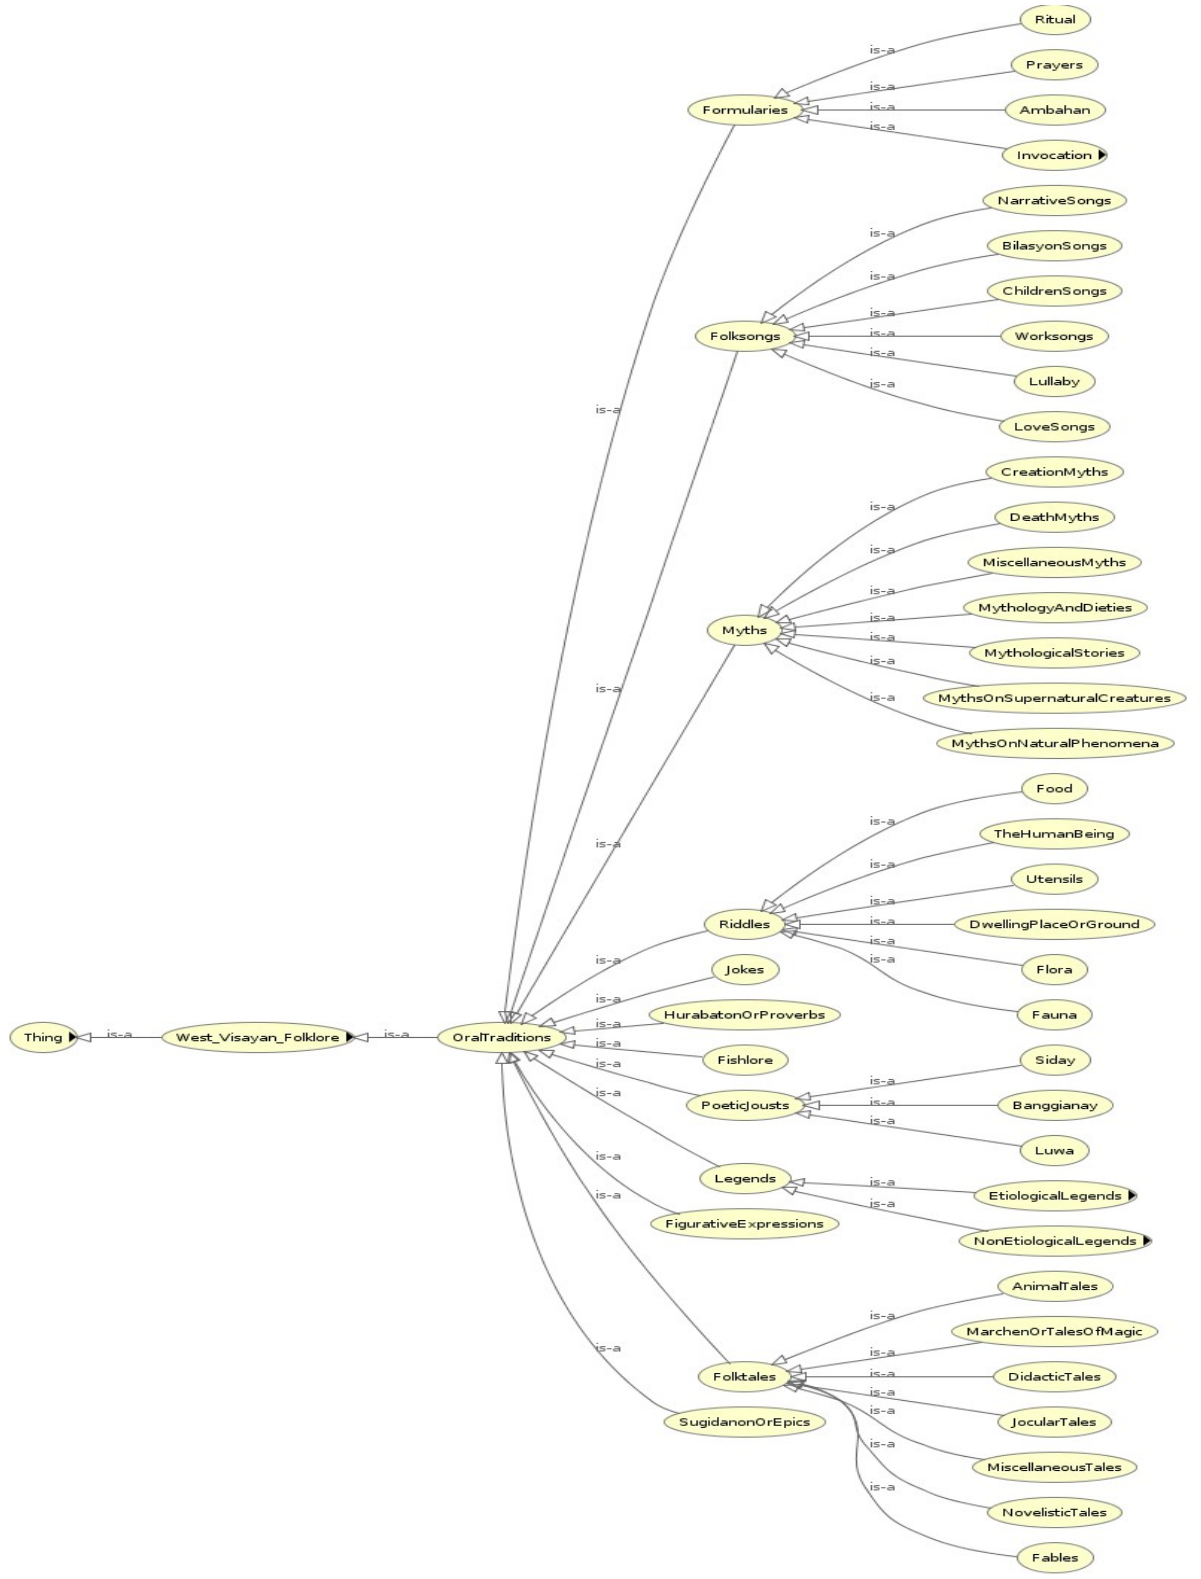
\includegraphics[width=\linewidth]{figures/Dimzon and Dimzon (2015) Ontology.png}
    \caption{Diagram of The Original Ontology by \protect\citeA{dimzon2015}}
    \label{fig:ontology diagram}
\end{figure}

As illustrated in Figure \ref{fig:ontology diagram}, the original ontology by \citeA{dimzon2015} does not contain story details but rather the classification of the different oral traditions found in the cultures of Western Visayas. This presents the knowledge gap that the researchers propose on exploring. Specifically, the ontology will be expanded with story elements for the Myths, Legends, and Folktales entities present in the current iteration of the ontology.  

\FloatBarrier

